\graphicspath{{images/}}

\section{Ход работы}

Я выбрал набор данных Beginner classification dataset \cite{kaggle} для выполнения лабораторной работы. В описании датасета предлагают самим 
"предстваить" целевую переменную. В качестве примера представим, что целевая переменная - успех изучения нового хобби.

Признаки в наборе данных:

\begin{enumerate}
    \item
    age --- возраст человека, который решил изучить новое хобби
    \item
    interest --- показатель его заинтересованности.
    \item
    success --- успех или неуспех изучения нового хобби.
\end{enumerate}

Перед выявлением зависимостей между признаками следует проверяю целостность набора данных:
\begin{alltt}
RangeIndex: 297 entries, 0 to 296
Data columns (total 3 columns):
 #   Column    Non-Null Count  Dtype  
---  ------    --------------  -----  
 0   age       297 non-null    float64
 1   interest  297 non-null    float64
 2   success   297 non-null    float64
dtypes: float64(3)
memory usage: 7.1 KB
\end{alltt}

В наборе нет неполных данных, а все признаки - числовые.
\pagebreak

Построю графики для каждой пары признаков. Синим отмечен успех, оранжевым - неуспех:
\begin{center}
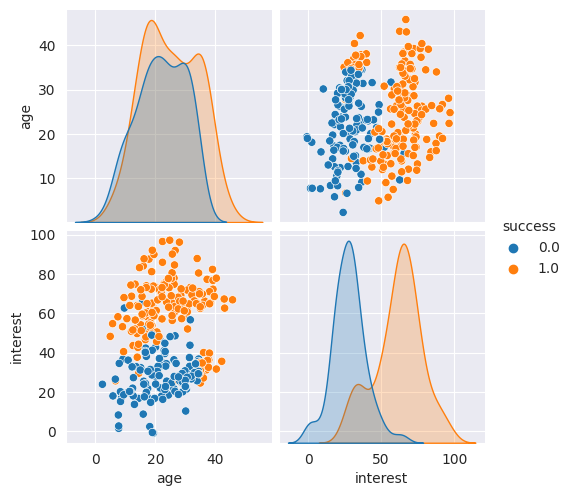
\includegraphics[scale=0.25]{pair}
\end{center}\pagebreak

Построю корреляционную матрицу для признаков:
\begin{center}
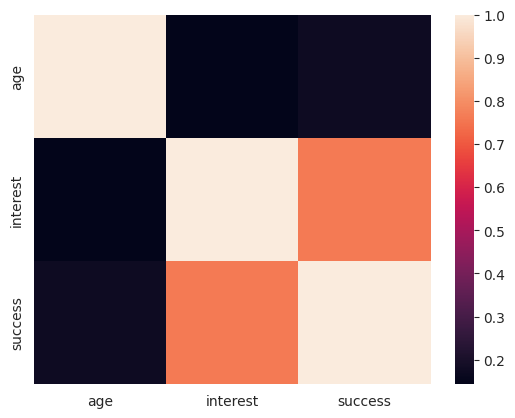
\includegraphics[scale=0.65]{corr}
\end{center}
Так же построю гистограммы для числовых признаков:
\begin{center}
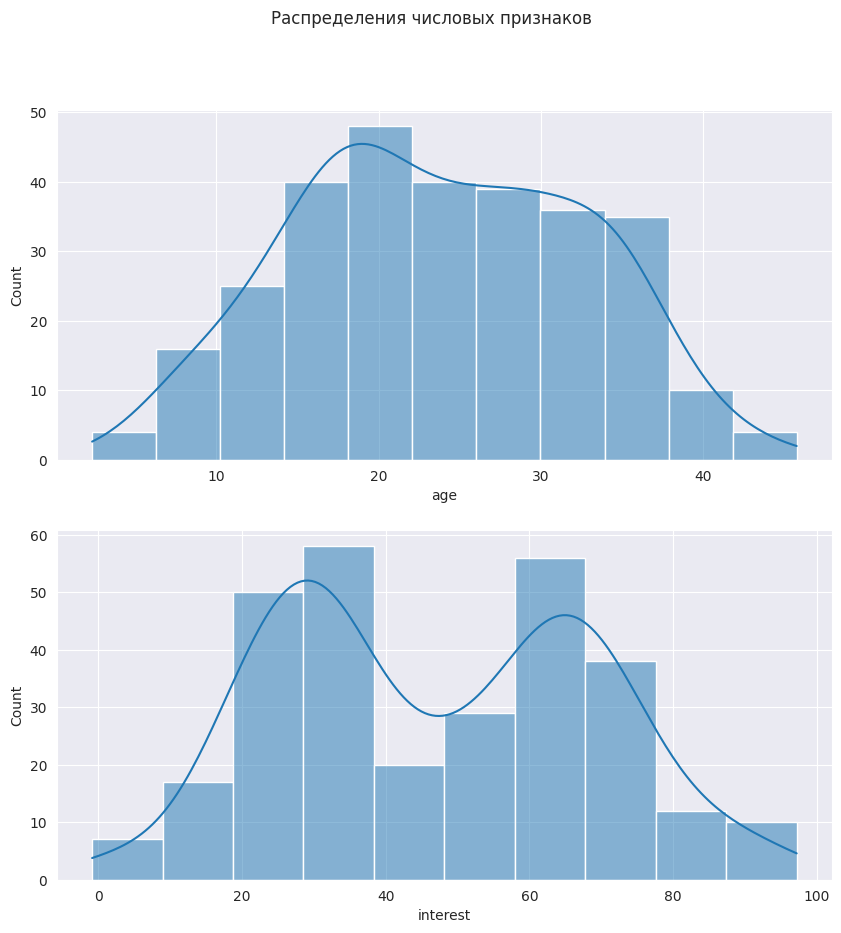
\includegraphics[scale=0.35]{bar}
\end{center}
Выбросов не было обнаружено, так как датасет довольно маленький.
\pagebreak

Соотношение классов объектов:
\begin{center}
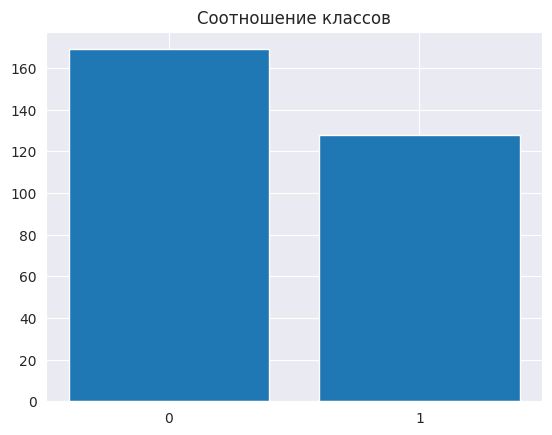
\includegraphics[scale=0.65]{classes}
\end{center}
Объектов разных классов примерно одинаковое количество, oversampling не требуется. Данные готовы к обучению.

\pagebreak
